% =====================================================================
%  Propagation operators on LEO ISL graphs: budget and t-parameterisation decide the ranking
%  Dich: Computer Communications (Elsevier, hybrid, KHONG gold OA)
%
%  ⛔ KHONG GO SO. Moi con so den tu ../figures/out/numbers.tex va tab*.tex, sinh boi
%     figures/make_figures.py tu code/results/grid12, grid3 va results-as-submitted.
%  ⛔ RANG BUOC TU claim-structure.md:
%   - KHONG "quantum-inspired" trong tieu de. KHONG chu "honest" o bat ky dau.
%   - Co che unitary la cua CTQW-GNN (arXiv:2608.20738); bai nay DO, khong nhan co che.
%   - TNSM dang phan bien: KHONG dung chung ma/du lieu/hinh, KHONG trich.
%   - Ban so bo 06/2026 chi duoc nhac nhu "preliminary version" kem repo, khong nhu bai da dang.
% =====================================================================
\documentclass[preprint,11pt,3p]{elsarticle}

\usepackage[T1]{fontenc}
\usepackage[utf8]{inputenc}
\usepackage{graphicx}
\usepackage{booktabs}
\usepackage{amsmath,amssymb}
\usepackage[hyphens]{url}
\usepackage{tikz}
\usetikzlibrary{arrows.meta,positioning,fit}
\usepackage[hidelinks]{hyperref}

\setcounter{topnumber}{3}
\setcounter{bottomnumber}{2}
\setcounter{totalnumber}{4}
\renewcommand{\topfraction}{0.9}
\renewcommand{\bottomfraction}{0.6}
\renewcommand{\textfraction}{0.07}
\renewcommand{\floatpagefraction}{0.75}

% GENERATED by figures/make_figures.py. Do not edit.
\newcommand{\numAboveHeatShellOne}{29}
\newcommand{\numAboveMaxGainPct}{18.3}
\newcommand{\numAboveWalkShellOne}{34}
\newcommand{\numAurcHeatRobust}{0}
\newcommand{\numAurcHeatWinsArm}{2}
\newcommand{\numAurcSigHolm}{0}
\newcommand{\numAurcSigRaw}{2}
\newcommand{\numAurcWalkRobust}{0}
\newcommand{\numAurcWalkWinsArm}{0}
\newcommand{\numCacheIdenticalDigits}{16}
\newcommand{\numCollapseGcn}{18/120}
\newcommand{\numCollapseGcnEscaped}{6}
\newcommand{\numCollapseHeat}{11/120}
\newcommand{\numCollapseHeatEscaped}{4}
\newcommand{\numCollapseWalk}{11/120}
\newcommand{\numCollapseWalkEscaped}{3}
\newcommand{\numCpuSecsLarge}{1096}
\newcommand{\numEscapeHeat}{45/79}
\newcommand{\numEscapeHeatPct}{57}
\newcommand{\numEscapePz}{0.95}
\newcommand{\numEscapeWalk}{46/80}
\newcommand{\numEscapeWalkPct}{58}
\newcommand{\numFeasibleNGpuMem}{19300}
\newcommand{\numFloorCellsLarge}{24}
\newcommand{\numGainDelaySmallMaxReleased}{19.5}
\newcommand{\numGainDelaySmallMaxSubmitted}{29.2}
\newcommand{\numGainDelaySmallMinReleased}{7.9}
\newcommand{\numGainDelaySmallMinSubmitted}{10.9}
\newcommand{\numGainHopsSmallMaxReleased}{28.7}
\newcommand{\numGainHopsSmallMaxSubmitted}{40.3}
\newcommand{\numGainHopsSmallMinReleased}{7.7}
\newcommand{\numGainHopsSmallMinSubmitted}{24.9}
\newcommand{\numGainLargeMax}{2.9}
\newcommand{\numGainLargeMaxReleased}{2.9}
\newcommand{\numGainLargeMaxSubmitted}{2.8}
\newcommand{\numGcnSdSmall}{0.012}
\newcommand{\numGridThreeArms}{2}
\newcommand{\numGridThreePathology}{40}
\newcommand{\numGridThreePathologyPct}{11.1}
\newcommand{\numGridThreeRiseMaxPct}{36}
\newcommand{\numGridThreeRuns}{360}
\newcommand{\numGridTwelveAbove}{84}
\newcommand{\numGridTwelveAtFloorLarge}{1352}
\newcommand{\numGridTwelveLargeRuns}{1436}
\newcommand{\numGridTwelvePathology}{5}
\newcommand{\numGridTwelvePlateau}{48}
\newcommand{\numGridTwelveRuns}{1920}
\newcommand{\numGthreeArmCells}{12}
\newcommand{\numGthreeCells}{6}
\newcommand{\numGthreeDelayDoubleRobust}{no}
\newcommand{\numGthreeDelayGainMax}{36}
\newcommand{\numGthreeDelayGainMin}{20}
\newcommand{\numGthreeDelayShellOneRobust}{heat}
\newcommand{\numGthreeDelaySmallRobust}{heat}
\newcommand{\numGthreeGcnGainDouble}{2.6}
\newcommand{\numGthreeGcnGainShellOne}{4.5}
\newcommand{\numGthreeGcnGainSmall}{27.6}
\newcommand{\numGthreeHeatRobust}{3}
\newcommand{\numGthreeHopsDoubleRobust}{no}
\newcommand{\numGthreeHopsGainMax}{69}
\newcommand{\numGthreeHopsGainMin}{15}
\newcommand{\numGthreeHopsShellOneRobust}{no}
\newcommand{\numGthreeHopsSmallConst}{0.189}
\newcommand{\numGthreeHopsSmallHeat}{0.058}
\newcommand{\numGthreeHopsSmallHeatSd}{0.005}
\newcommand{\numGthreeHopsSmallRobust}{heat}
\newcommand{\numGthreeHopsSmallWalk}{0.064}
\newcommand{\numGthreeHopsSmallWalkSd}{0.004}
\newcommand{\numGthreeLeadHeat}{7}
\newcommand{\numGthreeLeadWalk}{5}
\newcommand{\numGthreeRobustMaxPsign}{0.344}
\newcommand{\numGthreeRobustMinPsign}{0.016}
\newcommand{\numGthreeSigHolm}{0}
\newcommand{\numGthreeSigRaw}{5}
\newcommand{\numGthreeWalkLeadTie}{3}
\newcommand{\numGthreeWalkRobust}{0}
\newcommand{\numLargeSpreadMax}{0.002}
\newcommand{\numPprAlpha}{0.05}
\newcommand{\numPprK}{20}
\newcommand{\numPrelimHeatMAE}{0.168}
\newcommand{\numPrelimParams}{3301}
\newcommand{\numPrelimSeeds}{3}
\newcommand{\numPrelimWalkMAE}{0.148}
\newcommand{\numRankableCellsLarge}{0}
\newcommand{\numRankableLargeAtGFive}{0}
\newcommand{\numRankableLargeAtGOne}{5}
\newcommand{\numRankableLargeAtGTen}{0}
\newcommand{\numRankableLargeAtGTwo}{2}
\newcommand{\numReleasedParams}{612}
\newcommand{\numRobustHeatAtGFive}{3}
\newcommand{\numRobustHeatAtGOne}{3}
\newcommand{\numRobustHeatAtGTen}{3}
\newcommand{\numRobustHeatAtGTwo}{3}
\newcommand{\numSTwoSixFourCells}{8}
\newcommand{\numSTwoSixFourConst}{0.189}
\newcommand{\numSTwoSixFourHeatWins}{2}
\newcommand{\numSTwoSixFourTies}{5}
\newcommand{\numSTwoSixFourVerdictsReleased}{tie / tie / walk / tie}
\newcommand{\numSTwoSixFourVerdictsSubmitted}{tie / heat / tie / heat}
\newcommand{\numSTwoSixFourWalkWinP}{0.109}
\newcommand{\numSTwoSixFourWalkWins}{1}
\newcommand{\numSdRatioCells}{12}
\newcommand{\numSdRatioGeThree}{1}
\newcommand{\numSdRatioLtOne}{2}
\newcommand{\numSdRatioMedian}{1.42}
\newcommand{\numSecsGcnLarge}{21}
\newcommand{\numSecsHeatLarge}{81}
\newcommand{\numSecsWalkLarge}{169}
\newcommand{\numSgcK}{8}
\newcommand{\numSpreadExpHeat}{1.00}
\newcommand{\numSpreadExpWalk}{2.00}
\newcommand{\numSpreadFitTmax}{40}
\newcommand{\numSpreadFitTmin}{7}
\newcommand{\numSpreadResidHeat}{0.000}
\newcommand{\numSpreadResidWalk}{0.000}
\newcommand{\numSubmittedParams}{3301}
\newcommand{\numSwapCells}{12}
\newcommand{\numSwapCellsMovedTwoPlus}{4}
\newcommand{\numSwapMaxMoved}{3}
\newcommand{\numSwapMedianMoved}{1}
\newcommand{\numTlayerOneDoubleHeat}{10.6}
\newcommand{\numTlayerOneDoubleWalk}{2.3}
\newcommand{\numTlayerOneShellOneHeat}{8.2}
\newcommand{\numTlayerOneShellOneWalk}{1.9}
\newcommand{\numTlayerOneSmallHeat}{3.1}
\newcommand{\numTlayerOneSmallWalk}{1.3}


\newcommand{\Lap}{\mathbf{L}}
\newcommand{\Phiop}{\boldsymbol{\Phi}}

\journal{Computer Communications}

\begin{document}

\begin{frontmatter}

\title{Training Budget and Time Parameterisation Decide the Ranking of\\
Propagation Operators on LEO Inter-Satellite-Link Graphs}

\author[caira]{Phuc Hao Do\corref{cor1}}
\ead{haodp@dau.edu.vn}
\cortext[cor1]{Corresponding author.}
\affiliation[caira]{organization={CAIRA, Danang Architecture University},
  city={Da Nang}, country={Viet Nam}}

\begin{abstract}
Learned propagation on the inter-satellite-link graph of a low-Earth-orbit constellation is
increasingly proposed for routing, state estimation and resource management, and several
recent works argue that operators derived from continuous-time quantum walks reach farther
than diffusion and should therefore help most on large graphs. We test that argument under
controlled conditions. Three propagation operators that share one Laplacian eigenbasis and one
network, a local GCN step, the heat kernel $e^{-t\Lap}$ and the quantum-walk probability
kernel $|e^{-it\Lap}|^{2}$, are compared on Walker-delta shells of 264 to 4400 satellites,
on two node-field tasks, over ten seeds, and across arms that vary the parameterisation and
initialisation of the learned propagation time $t$, the network capacity and the training
budget, for \numGridTwelveRuns{} plus \numGridThreeRuns{} training runs on one machine.
Three findings follow. First, with a training budget held fixed across scales, no operator
improves on a constant predictor by more than \numGainLargeMaxSubmitted\% on any shell of
1584 satellites or more, in any arm: the comparison there measures a budget floor, not an
operator. Second, on the one scale where learning occurs under that budget, the ranking of
the two spectral operators changes with how $t$ is parameterised and initialised, and traces
to a seed-level bimodality in which a run either leaves the constant solution or does not.
Third, with a five-fold budget every shell leaves the floor, and wherever the comparison is
decidable the heat kernel matches or beats the walk kernel, with seed variance several times
smaller; the walk kernel wins robustly in none of \numGthreeCells{} task-scale cells. Long
training at a fixed learning rate also collapses \numGridThreePathologyPct\% of runs back to
the constant solution. A preliminary version of this study reported a walk-kernel advantage at
1584 satellites from \numPrelimSeeds{} seeds; that result is not reproduced, and its released
artifact used a different configuration from its text. All code, results and the declared
protocol are released.
\end{abstract}

\begin{keyword}
LEO constellations \sep inter-satellite links \sep graph neural networks \sep
spectral propagation \sep quantum walks \sep evaluation methodology \sep reproducibility
\end{keyword}

\end{frontmatter}

% =====================================================================
\section{Introduction}

The inter-satellite-link (ISL) graph of a low-Earth-orbit (LEO) mega-constellation is large,
nearly regular, and changes with time as satellites move and links across the seam and the
polar regions come and go~\cite{plusgrid,starlink}. Learned models that propagate information
over this graph have been proposed for routing~\cite{lira,deepladu}, connectivity and
multi-connectivity decisions~\cite{comsat}, and related network functions. Most of them are
graph neural networks, and a graph neural network is, at each layer, a propagation operator
$\Phiop(\Lap)$ applied to node features followed by a shared nonlinearity~\cite{gcn,shuman}.
Which operator to use is therefore a design decision with consequences at constellation scale.

Three operators span the design space that this paper studies. The local step of a graph
convolutional network~\cite{gcn}, equation~\eqref{eq:gcn} below, moves information one hop per layer. The heat kernel
$e^{-t\Lap}$ moves it diffusively, over a range that grows like $\sqrt{t}$~\cite{grand}. The
continuous-time quantum walk~\cite{farhi} evolves $e^{-it\Lap}$ unitarily and spreads
ballistically, over a range that grows like $t$; its transition-probability kernel
$|e^{-it\Lap}|^{2}$ is a real, row-stochastic matrix that can be dropped into the same layer
in place of the heat kernel~\cite{qwnn,qgnn}. Recent work has turned the ballistic property
into an argument: because the unitary propagator damps no frequency and preserves feature
norm, walk-based operators should resist over-smoothing and help most where geodesics are
long~\cite{ctqwgnn,ctqwformer,graphqwalk}. LEO ISL graphs, whose diameter grows with the
number of satellites, are a natural place to look for that benefit.

A preliminary version of this study, circulated for review in June 2026 and available in the
companion repository, looked and reported finding it: on a 1584-satellite shell the walk
kernel reached a mean absolute error of \numPrelimWalkMAE{} against \numPrelimHeatMAE{} for the
heat kernel, from \numPrelimSeeds{} seeds, and the trend from smaller shells was read as the
ballistic mechanism emerging with scale. This paper asks whether that ranking is a property of
the operators or of the evaluation, and answers by controlling the evaluation.

The reason to suspect the evaluation is that three quantities were left implicit in the
preliminary comparison and in most comparisons of this kind. The first is the training budget:
if the number of epochs is held fixed while the graph grows, a model may simply not have left
the constant solution on the large graph, and a comparison between two operators that have
both failed to learn measures noise. The second is the learned propagation time $t$: both
spectral operators carry a per-layer $t$ that is trained by gradient descent, and how it is
parameterised and where it starts determines how far each operator can reach and whether it
can reach at all. The third is the number of seeds, which decides whether a difference is
distinguishable from run-to-run variation. We make all three explicit and vary them.

The contribution is a controlled comparison and what it shows.
\begin{itemize}
\item A protocol in which the three operators share one eigendecomposition, one network, one
  parameter count and one training loop, and in which the training budget, the $t$
  parameterisation and initialisation, the network capacity and the seed count are arms of the
  study rather than fixed choices. Every rule for reading the results, including the constant
  baseline, the floor below which a cell is not rankable, the seed-majority needed to call a
  winner, and the requirement that a ranking hold in every arm, was declared before the runs
  and is recorded in the repository history.
\item Under a fixed budget of 200 epochs, no operator improves on the constant predictor by
  more than \numGainLargeMaxSubmitted\% on any shell of 1584 satellites or more, in any of eight
  configuration-by-arm combinations (Section~\ref{sec:floor}). On the one shell where learning
  occurs, the heat-versus-walk ranking changes with the $t$ arm, and the reason is visible at
  the seed level: a run either leaves the constant solution or stays on it
  (Section~\ref{sec:hidden}).
\item With a budget of 1000 epochs every shell leaves the floor. Wherever the comparison is
  decidable under the declared rules, the heat kernel matches or beats the walk kernel, with
  seed variance several times smaller, and the walk kernel wins in none of \numGthreeCells{}
  task-scale cells (Section~\ref{sec:budget}). Long training at a fixed learning rate collapses
  \numGridThreePathologyPct\% of runs back to the constant solution, which the protocol counts
  rather than drops.
\item The preliminary result is not reproduced under this protocol, and the released artifact
  of the preliminary version turns out to have used a network of \numPrelimParams{} parameters
  while its released code defaults to \numReleasedParams{}, with no script for the experiment in
  question (Section~\ref{sec:threats}). We report this because it is the kind of gap the
  protocol is designed to close.
\end{itemize}

The rest of the paper is organised as follows. Section~\ref{sec:related} places the operators
and the LEO setting in the literature. Section~\ref{sec:setting} defines the graphs (Section~\ref{sec:graphs}), the three
operators on one eigenbasis (Section~\ref{sec:operators}) and the network and tasks
(Section~\ref{sec:network}). Section~\ref{sec:protocol} states the protocol and the reading rules
(Section~\ref{sec:rules}).
Section~\ref{sec:results} reports the three grids. Section~\ref{sec:discussion} interprets
them, Section~\ref{sec:threats} lists what limits them, and Section~\ref{sec:conclusion}
concludes.

% =====================================================================
\section{Related work}
\label{sec:related}

\paragraph{Propagation operators and their reach}
Spectral graph convolutions began as polynomial filters of the Laplacian~\cite{chebnet,shuman};
the graph convolutional network of Kipf and Welling~\cite{gcn} keeps the first-order term and
applies a normalised adjacency once per layer, so depth bounds reach. Stacking layers drives
features toward a constant, the over-smoothing effect identified by Li et al.~\cite{lihanwu},
shown by Oono and Suzuki~\cite{oono} to be exponential in depth, and surveyed by Rusch et
al.~\cite{oversmooth}; remedies include decoupling propagation from transformation as in
SGC~\cite{sgc} and personalised-PageRank propagation~\cite{appnp}, and residual and identity
terms as in GCNII~\cite{gcnii}. Alon and Yahav~\cite{oversquash} describe the complementary
bottleneck by which information from exponentially many distant nodes is squashed into
fixed-size vectors, which Topping et al.~\cite{topping} relate to negative curvature of the
graph. Continuous-time views
replace the discrete step with a differential equation on the graph: GRAND~\cite{grand} uses
diffusion, whose solution is the heat kernel; PDE-GCN~\cite{pdegcn} and graph-coupled
oscillator networks~\cite{graphcon} use wave-type dynamics, whose reach grows linearly in
time rather than as a square root. The distinction between diffusive and ballistic spreading
that motivates the walk kernel in this paper is the same distinction, and the wave-type models
are its classical form.

\paragraph{Quantum walks as graph operators}
The continuous-time quantum walk of Farhi and Gutmann~\cite{farhi} evolves an amplitude
vector by $e^{-it\Lap}$ and spreads ballistically; Kempe~\cite{kempe} and M\"ulken and
Blumen~\cite{mulken} review the walk and its transport properties on complex networks, and
Childs~\cite{childs} shows it is computationally universal. Dernbach et al.~\cite{qwnn} and Verdon et
al.~\cite{qgnn} were among the first to place walk-derived operators inside trainable graph
models. GraphQWalk~\cite{graphqwalk} builds unsupervised, position-independent structural
embeddings from walk transition probabilities. CTQWformer~\cite{ctqwformer} learns the walk
Hamiltonian and feeds final-time probabilities into a graph transformer. CTQW-GNN~\cite{ctqwgnn}
uses the unitary propagator itself in feature space and proves that, because its eigenvalues lie
on the unit circle, no frequency is damped and the Dirichlet energy of the features cannot decay
exponentially with depth. That result concerns the unitary operator acting on features. The
operator studied here is the transition-probability kernel $|e^{-it\Lap}|^{2}$, a real
nonnegative matrix that shares the ballistic profile of the walk but not the norm-preserving
property; the distinction matters for interpreting the results
(Section~\ref{sec:discussion}). Quantum walks on communication networks have also been used
directly, for instance the Hadamard-walk model for network identification of
Liang et al.~\cite{hadamard}.

\paragraph{Graph learning on LEO constellations}
Handley~\cite{handley} first argued that inter-satellite routing in a mega-constellation is
a latency question, Bhattacherjee and Singla~\cite{plusgrid} fix the +Grid inter-satellite
topology that most later work assumes, Kassing et al.~\cite{hypatia} provide the Hypatia
simulator for such networks, and del Portillo et al.~\cite{starlink} compare the announced
constellations, including the Starlink shell whose geometry the 1584-satellite graph here
reproduces. Learned models on this graph include the link-identified routing architecture of
Zhang et al.~\cite{lira}, the duality-guided graph learning for joint connectivity and routing
of Gu et al.~\cite{deepladu}, and machine-learning-driven cellular-satellite
multi-connectivity~\cite{comsat}. None of these compares propagation operators under a common
parameterisation of reach, which is the gap this study addresses. The tasks used here are
deliberately decoupled from any particular routing or traffic-engineering system, so that the
propagation question is isolated from questions of load.

\paragraph{Evaluation pitfalls}
Shchur et al.~\cite{shchur} showed that the ranking of graph neural network architectures on
standard benchmarks changes with the data split and the seed, Henderson et al.~\cite{henderson}
made the corresponding point for deep reinforcement learning, where few seeds and unreported
tuning produce rankings that do not replicate, Bouthillier et al.~\cite{bouthillier} quantify
how much benchmark variance comes from sources other than the method, and Pineau et
al.~\cite{pineau} report on the reproducibility programme that turned such findings into
checklists. The present study applies the same discipline
to a comparison of propagation operators, and adds two quantities specific to spectral
operators, the training budget relative to graph size and the parameterisation of the
learned propagation time.

% =====================================================================
\section{Setting}
\label{sec:setting}

\subsection{Constellation graphs}
\label{sec:graphs}

Each graph is a snapshot of a Walker-delta shell. Satellite positions follow circular-orbit
propagation in an Earth-centred inertial frame; inter-satellite links follow the +Grid
pattern~\cite{plusgrid}, two intra-plane and two inter-plane links per satellite, with
inter-plane links suppressed above 70$^{\circ}$ latitude and across the counter-rotating seam.
The graph is restricted to its largest connected component. Four shells are used
(Table~\ref{tab:shells}). The 264-satellite shell is the main scale of the preliminary
version; the 1584-satellite shell reproduces the geometry of the first Starlink
shell~\cite{starlink}, 72 planes of 22 satellites at 53$^{\circ}$ and 550~km; the 3168- and
4400-satellite shells are scale-ups of that geometry, 72 planes of 44 and 100 planes of 44,
and are synthetic in the sense that no operator flies them. They exist to make the diameter
grow.

\begin{table}[t]
\centering
\caption{The four shells. All use +Grid links, a 70$^{\circ}$ polar cutoff and a seam cut. The two largest are scale-ups of the Starlink
shell-1 geometry and are not deployed constellations.}
\label{tab:shells}
% GENERATED by figures/make_figures.py
\begin{tabular}{@{}rrrrrl@{}}
\toprule
satellites & planes & per plane & incl.\ ($^{\circ}$) & alt.\ (km) & note \\
\midrule
264 & 24 & 11 & 53 & 550 & main scale of the preliminary version \\
1584 & 72 & 22 & 53 & 550 & Starlink shell-1 geometry~\cite{starlink} \\
3168 & 72 & 44 & 53 & 550 & scale-up, synthetic \\
4400 & 100 & 44 & 53 & 550 & scale-up, synthetic \\
\bottomrule
\end{tabular}

\end{table}

Each training or evaluation instance draws a snapshot time uniformly over the orbital period
and a destination satellite uniformly over the component. Instance construction is seeded, so
every instance is reproducible from its index.

\subsection{Three operators on one eigenbasis}
\label{sec:operators}

Let $\Lap = \mathbf{D} - \mathbf{A}$ be the combinatorial Laplacian of the snapshot, with
eigendecomposition $\Lap = \mathbf{U}\,\mathrm{diag}(\lambda)\,\mathbf{U}^{\top}$ computed once
per instance and shared by all operators. The three operators are
\begin{align}
\Phiop_{\mathrm{gcn}} &= \tilde{\mathbf{D}}^{-1/2}(\mathbf{A}+\mathbf{I})\tilde{\mathbf{D}}^{-1/2}, \label{eq:gcn}\\
\Phiop_{\mathrm{heat}}(t) &= \mathbf{U}\,\mathrm{diag}\!\left(e^{-t\lambda}\right)\mathbf{U}^{\top}
  = e^{-t\Lap}, \label{eq:heat}\\
\Phiop_{\mathrm{walk}}(t) &= \left|\mathbf{U}\,\mathrm{diag}\!\left(e^{-it\lambda}\right)\mathbf{U}^{\top}\right|^{2}
  = \left|e^{-it\Lap}\right|^{2}, \label{eq:walk}
\end{align}
where the square in~\eqref{eq:walk} is taken entrywise on the modulus, so that
$[\Phiop_{\mathrm{walk}}]_{ij}$ is the probability that a continuous-time quantum walk started
at $j$ is found at $i$ after time $t$. Both~\eqref{eq:heat} and~\eqref{eq:walk} are real,
nonnegative and row-stochastic; they differ in the profile of the row as a function of graph
distance, monotone for the heat kernel and oscillatory for the walk kernel, and in how that
profile's width grows with $t$.

\subsection{Network, parameterisation of $t$, and tasks}
\label{sec:network}

The network has $K$ layers, each computing
$\mathbf{H}^{(\ell+1)} = \sigma\!\left(\Phiop^{(\ell)}\,\mathbf{H}^{(\ell)}\mathbf{W}^{(\ell)}\right)$
with a ReLU nonlinearity and a linear read-out to one scalar per node. For the two spectral
operators, each layer carries its own scalar propagation time $t_{\ell}$, trained jointly with
the weights. The preliminary version parameterised it as $t_{\ell}=\mathrm{relu}(\theta_{\ell})$
with $\theta_{\ell}$ initialised at 0.5. Section~\ref{sec:protocol} explains why this is an arm
of the present study and adds $t_{\ell}=\mathrm{softplus}(\theta_{\ell})$, which keeps
$t_{\ell}>0$ with a live gradient, initialised so that the two parameterisations start at the
same value. The GCN operator has no $t$.

The input to every node is two features, an indicator of the destination and the normalised
degree. Two node-field targets are used. With $d$ the destination, $h(i,d)$ the geodesic hop count
and $\tau(i,d)$ the shortest-path propagation delay computed on the inter-satellite link
lengths, the targets are
\begin{equation}
y^{\mathrm{hop}}_{i} = \frac{h(i,d)}{\max_{j} h(j,d)}, \qquad
y^{\mathrm{delay}}_{i} = \frac{\tau(i,d)}{\max_{j} \tau(j,d)},
\label{eq:tasks}
\end{equation}
so that both lie in $[0,1]$ and the constant predictor has the same meaning on every shell. The
hop field is the task of the preliminary version. Both fields in~\eqref{eq:tasks}
require the model to move a single seeded signal across the graph, which is the propagation
question in isolation; neither involves traffic or load. The metric is the mean absolute
error (MAE) over nodes on held-out instances.

% =====================================================================
\section{Protocol}
\label{sec:protocol}

\subsection{Parameter matching and the arms}

The three operators share depth, width, weight shapes and training loop, so a difference in
error is attributable to the operator and not to capacity. Two capacities are used: width 16
with three layers, which is the default of the released code of the preliminary version
(\numReleasedParams{} parameters including the $t_{\ell}$), and width 32 with four layers, which
the text of the preliminary version describes and its released results were produced with
(\numSubmittedParams{} parameters). Adam~\cite{adam} at learning rate 0.01, eight training and
six evaluation instances per seed, and full-batch updates are used throughout.

Four quantities are arms rather than fixed choices.
\begin{itemize}
\item \textbf{Parameterisation of $t$.} A pilot run under the released parameterisation showed
  the learned $t_{\ell}$ going negative in the second and third layers, where
  $\mathrm{relu}(t_{\ell})=0$ turns the propagator into the identity and stops its gradient, so
  that a model reported as three or four layers of spectral propagation was propagating in one.
  The softplus parameterisation removes this; the relu parameterisation is kept as a control so
  that the preliminary configuration is one of the arms.
\item \textbf{Initialisation of $t$.} $t_{0}\in\{0.5, 2\}$, since the same pilot showed the
  learned reach, and with it the operator ranking, depending on where $t$ starts.
\item \textbf{Capacity.} The two configurations above.
\item \textbf{Budget.} 200 epochs, the preliminary value, held fixed across scales; and 1000
  epochs for the second grid.
\end{itemize}
Grid 1 runs both capacities, all four $t$ arms, four shells, two tasks, three operators and ten
seeds at 200 epochs (\numGridTwelveRuns{} runs). Grid 2 runs the width-32 configuration at 1000
epochs on the three smaller shells with the two $t_{0}=0.5$ arms (\numGridThreeRuns{} runs).
All runs were executed on one machine, one GPU per arm, with the eigendecomposition of each
instance cached and shared so that every arm sees bit-identical eigenpairs.

\subsection{Reading rules, declared before the runs}
\label{sec:rules}

Five rules govern how a cell, one (task, shell, arm) combination, is read. They were fixed
before the first grid was launched, and two of them were tightened after the first runs
exposed a gap; both changes are dated in the repository and stated here.
\begin{enumerate}
\item \textbf{Constant baseline.} Every cell reports the MAE of the predictor that outputs the
  mean of the target. Whether an operator beats it is a result, never a filter.
\item \textbf{Pathology.} A run is excluded only for a training pathology: a non-finite loss,
  or a loss that rises by more than 1\% between successive thirds of training. Excluded runs
  are counted next to every number they affect. A run whose loss is flat from the start because
  it sits on the constant solution is a \emph{plateau}, a legitimate outcome, and is kept. The
  first draft of this rule required a 10\% loss drop and would have discarded plateaus as
  failures; the draft was corrected when the first grid produced them.
\item \textbf{Floor.} Let $\bar{e}_{\mathrm{op}}$ be the mean MAE of an operator over its
  valid seeds in a cell and $\bar{e}_{0}$ that of the constant predictor. The cell's gain is
  \begin{equation}
  g = \frac{\bar{e}_{0} - \min_{\mathrm{op}} \bar{e}_{\mathrm{op}}}{\bar{e}_{0}},
  \label{eq:gain}
  \end{equation}
  and the cell is \emph{rankable} only if $g \geq 0.05$. Below that, differences between operators are within the
  band in which no operator has learned, and the cell is reported as a floor. This rule was
  added after the first completed cells, all on the 4400-satellite shell, showed the three
  operators' means within \numLargeSpreadMax{} of one another and of the constant baseline
  while the seed-majority rule below still declared a winner.
\item \textbf{Winner.} Within a rankable cell, with $S$ the set of seeds valid for both
  spectral operators and $e_{\mathrm{op},s}$ the MAE of seed $s$, the heat kernel wins if
  \begin{equation}
  \bar{e}_{\mathrm{heat}} < \bar{e}_{\mathrm{walk}}
  \quad\text{and}\quad
  \bigl|\{ s \in S : e_{\mathrm{heat},s} < e_{\mathrm{walk},s} \}\bigr| \geq 7,
  \label{eq:win}
  \end{equation}
  and symmetrically for the walk kernel; otherwise the cell is a tie. Fewer than seven valid
  seed pairs, $|S|<7$, leaves the cell undecided.
\item \textbf{Robustness.} A ranking at a (task, shell) is claimed only if it is the same in
  every $t$ arm run at that budget.
\end{enumerate}
The rules are implemented once, in the analysis script that produces every table and figure,
and the same script prints the pathology and plateau counts beside every mean.
Figure~\ref{fig:protocol} summarises the grids and the reading rules, and
Table~\ref{tab:summary} collects the headline numbers with the section that derives each.

\begin{figure}[t]
\centering
% GENERATED by figures/make_figures.py
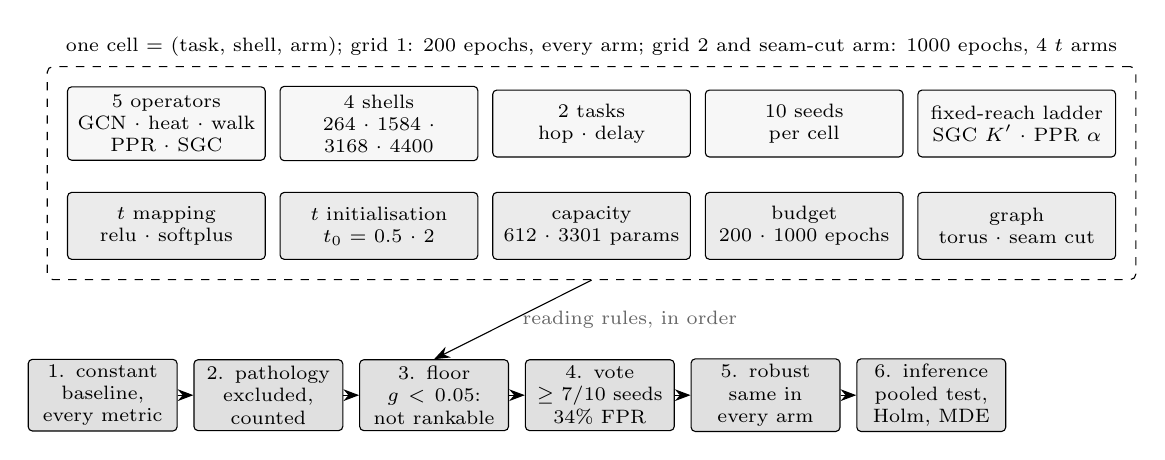
\begin{tikzpicture}[
  font=\scriptsize,
  box/.style={draw, rounded corners=1.5pt, align=center, inner sep=3pt, minimum height=8.5mm, text width=23mm},
  dim/.style={box, fill=black!3}, arm/.style={box, fill=black!8},
  rule/.style={box, text width=17.5mm, minimum height=9mm, fill=black!12, inner sep=2pt},
  >={Stealth[length=2mm]}]
\node[dim] (ops)    at (0,0)      {5 operators\\GCN $\cdot$ heat $\cdot$ walk\\PPR $\cdot$ SGC};
\node[dim] (shells) at (2.7,0)    {4 shells\\264 $\cdot$ 1584 $\cdot$ 3168 $\cdot$ 4400};
\node[dim] (tasks)  at (5.4,0)    {2 tasks\\hop $\cdot$ delay};
\node[dim] (seeds)  at (8.1,0)    {10 seeds\\per cell};
\node[arm] (tp)     at (0,-1.3)   {$t$ mapping\\relu $\cdot$ softplus};
\node[arm] (t0)     at (2.7,-1.3) {$t$ initialisation\\$t_{0}$ = 0.5 $\cdot$ 2};
\node[arm] (cap)    at (5.4,-1.3) {capacity\\612 $\cdot$ 3301 params};
\node[arm] (ep)     at (8.1,-1.3) {budget\\200 $\cdot$ 1000 epochs};
\node[arm] (gr)     at (10.8,-1.3) {graph\\torus $\cdot$ seam cut};
\node[dim] (fx)     at (10.8,0)    {fixed-reach ladder\\SGC $K'$ $\cdot$ PPR $\alpha$};
\node[draw, dashed, rounded corners=2pt, inner sep=2.5mm, fit=(ops)(seeds)(tp)(ep)(gr)(fx)] (grid) {};
\node[anchor=south, font=\scriptsize] at (grid.north) {one cell = (task, shell, arm); grid 1: 200 epochs, every arm; grid 2 and seam-cut arm: 1000 epochs, 4 $t$ arms};
\node[rule] (r3) at (3.4,-3.45) {3. floor\\$g < 0.05$:\\not rankable};
\node[rule, left=2mm of r3] (r2) {2. pathology\\excluded,\\counted};
\node[rule, left=2mm of r2] (r1) {1. constant\\baseline,\\every metric};
\node[rule, right=2mm of r3] (r4) {4. vote\\$\geq 7/10$ seeds\\34\% FPR};
\node[rule, right=2mm of r4] (r5) {5. robust\\same in\\every arm};
\node[rule, right=2mm of r5] (r6) {6. inference\\pooled test,\\Holm, MDE};
\draw[->] (grid.south) -- node[right, font=\scriptsize, text=black!60] {reading rules, in order} (r3.north);
\draw[->] (r1) -- (r2); \draw[->] (r2) -- (r3); \draw[->] (r3) -- (r4); \draw[->] (r4) -- (r5); \draw[->] (r5) -- (r6);
\end{tikzpicture}

\caption{The study design. Every cell of the grid, one (task, shell, arm), runs the three
operators on the same instances and seeds; the five reading rules are applied in order by one
script, and a ranking is reported only if it survives all five.}
\label{fig:protocol}
\end{figure}

\begin{table}[t]
\centering
\caption{Headline numbers and where each is derived. Every value is generated from the result
files by the same script that produces the figures.}
\label{tab:summary}
% GENERATED by figures/make_figures.py
\begin{tabular}{@{}p{0.52\textwidth}lp{0.19\textwidth}@{}}
\toprule
finding & value & derived in \\
\midrule
runs, fixed 200-epoch budget (grid 1) & 1920 & Sec.~\ref{sec:floor} \\
largest gain over constant on any shell $\geq$1584, any arm, either capacity (grid 1) & 2.9\% & Fig.~\ref{fig:floor}, Tab.~\ref{tab:floor} \\
rankable cells at $\geq$1584 satellites, hop field, at floor 5\% / 2\% / 1\% (grid 1) & 0 / 2 / 5 of 24 & Tab.~\ref{tab:sens} \\
heat-vs-walk verdicts at 264 satellites across the four $t$ arms, submitted capacity (grid 1) & tie / heat / tie / heat & Fig.~\ref{fig:arms} \\
the same, released capacity (grid 1) & tie / tie / walk / tie & Tab.~\ref{tab:s264} \\
runs, 1000-epoch budget, 2 $t$ arms (grid 2) & 360 & Sec.~\ref{sec:budget} \\
task-scale cells where heat / walk wins in every arm, MAE (grid 2) & 3 / 0 of 6 & Tab.~\ref{tab:grid3} \\
the same on the far-node metric (grid 2) & 0 / 0 of 6 & Tab.~\ref{tab:aurc} \\
arm-level cells where heat / walk leads in mean, MAE (grid 2) & 7 / 5 of 12 & Tab.~\ref{tab:grid3} \\
arm-level cells with Wilcoxon $p<0.05$ before / after Holm, MAE (grid 2) & 5 / 0 of 12 & Tab.~\ref{tab:grid3inf} \\
runs collapsing to the constant solution under long training (grid 2) & 40 (11.1\%) & Sec.~\ref{sec:collapse} \\
preliminary 1584-satellite result, walk vs heat, 3 seeds & 0.148 vs 0.168 & Sec.~\ref{sec:budget} \\
\bottomrule
\end{tabular}

\end{table}

% =====================================================================
\section{Results}
\label{sec:results}

\subsection{A fixed budget produces a floor at scale}
\label{sec:floor}

Figure~\ref{fig:floor} and Table~\ref{tab:floor} show, for each capacity and each $t$ arm, the
gain~\eqref{eq:gain} of the best operator over the constant predictor as the shell grows, at the
preliminary budget of 200 epochs. On the 264-satellite shell the improvement is between
\numGainSTwoSixFourMinReleased\% and \numGainSTwoSixFourMaxReleased\% at the released capacity
and between \numGainSTwoSixFourMinSubmitted\% and \numGainSTwoSixFourMaxSubmitted\% at the
submitted capacity. On every larger shell it never exceeds \numGainLargeMaxSubmitted\%, in any
of the eight capacity-by-arm combinations, on either task: of the \numFloorCellsLarge{} hop-field
cells at 1584 satellites and above, \numRankableCellsLarge{} are rankable. The models have not
left the constant solution. Of \numGridTwelveRuns{} runs, \numGridTwelvePathology{} were excluded
as pathologies and \numGridTwelvePlateau{} on the large shells were plateaus in the sense of
rule~2.

\begin{figure}[t]
\centering
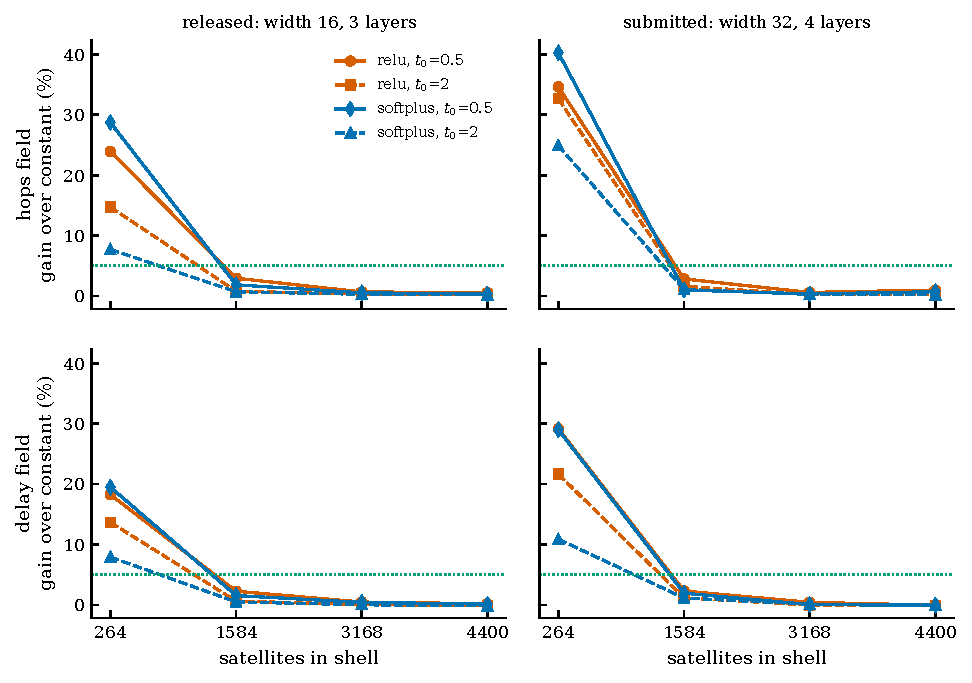
\includegraphics[width=\textwidth]{../figures/out/fig1-floor.pdf}
\caption{Improvement of the best operator over the constant predictor on the hop field at 200
epochs, as a function of shell size, for the released and the submitted capacity and the four
$t$ arms. The dotted line is the 5\% floor of rule~3. Above 264 satellites every combination
lies below it.}
\label{fig:floor}
\end{figure}

\begin{table}[t]
\centering
\caption{Improvement (\%) of the best operator over the constant predictor, hop field, 200
epochs, ten seeds per cell. A dagger marks cells below the 5\% floor, where the operator
ranking is not read.}
\label{tab:floor}
% GENERATED by figures/make_figures.py
\begin{tabular}{@{}llrrrr@{}}
\toprule
config & $t$ arm & 264 & 1584 & 3168 & 4400 \\
\midrule
released & relu, $t_0{=}$0.5 & 23.9 & 2.9$^{\dagger}$ & 0.7$^{\dagger}$ & 0.5$^{\dagger}$ \\
released & relu, $t_0{=}$2 & 14.7 & 0.8$^{\dagger}$ & 0.3$^{\dagger}$ & 0.2$^{\dagger}$ \\
released & softplus, $t_0{=}$0.5 & 28.7 & 1.8$^{\dagger}$ & 0.5$^{\dagger}$ & 0.3$^{\dagger}$ \\
released & softplus, $t_0{=}$2 & 7.7 & 0.7$^{\dagger}$ & 0.3$^{\dagger}$ & 0.2$^{\dagger}$ \\
submitted & relu, $t_0{=}$0.5 & 34.6 & 2.8$^{\dagger}$ & 0.6$^{\dagger}$ & 1.0$^{\dagger}$ \\
submitted & relu, $t_0{=}$2 & 32.7 & 1.6$^{\dagger}$ & 0.2$^{\dagger}$ & 0.2$^{\dagger}$ \\
submitted & softplus, $t_0{=}$0.5 & 40.3 & 0.9$^{\dagger}$ & 0.3$^{\dagger}$ & 0.7$^{\dagger}$ \\
submitted & softplus, $t_0{=}$2 & 24.9 & 1.1$^{\dagger}$ & 0.3$^{\dagger}$ & 0.2$^{\dagger}$ \\
\bottomrule
\end{tabular}

\end{table}

Doubling the width and adding a layer does not change this: the submitted capacity is as far
below the floor at 1584 satellites as the released one. Nor does the $t$ arm. The floor is
therefore not a capacity effect and not a parameterisation effect; Section~\ref{sec:budget}
shows that it is a budget effect.

\subsection{The propagation time is a hidden variable}
\label{sec:hidden}

On the 264-satellite shell, where learning does occur at 200 epochs, the ranking between the
two spectral operators is not stable. Figure~\ref{fig:arms} plots every seed for the submitted
capacity under the four $t$ arms. The declared verdicts read, in arm order,
\numSTwoSixFourVerdicts{}: the same operators on the same instances rank differently depending
only on how $t$ is parameterised and where it starts, so no ranking is claimed at this scale
(rule~5).

\begin{figure}[t]
\centering
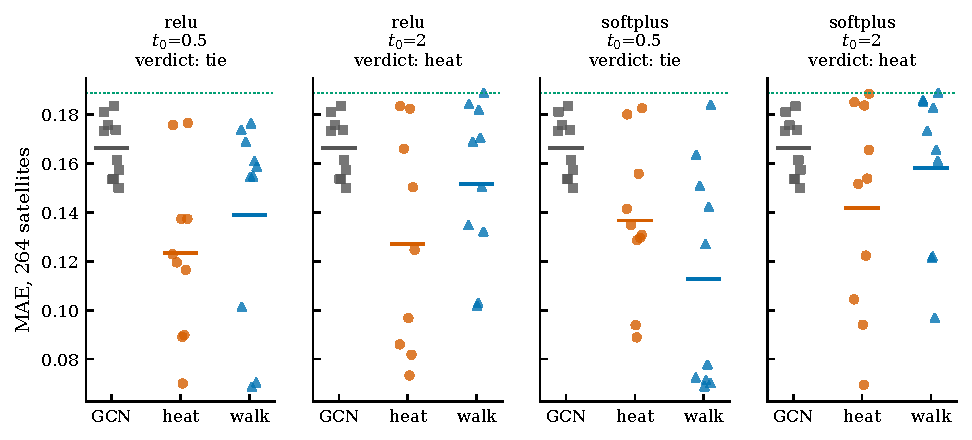
\includegraphics[width=\textwidth]{../figures/out/fig2-s264-arms.pdf}
\caption{Per-seed MAE on the hop field, 264 satellites, submitted capacity, 200 epochs, for
the four $t$ arms. Bars are means over valid seeds; the dotted line is the constant predictor.
The two spectral operators are bimodal across seeds: a run either leaves the constant solution
or stays near it.}
\label{fig:arms}
\end{figure}

The figure also shows why. For both spectral operators the ten seeds do not scatter around a
mean; they split. Some runs reach errors well below the constant predictor and the rest stay
near it. A ranking between two operators at this budget is largely a count of how many seeds
escaped, and that count moves with the $t$ arm because $t$ decides how far a layer reaches at
initialisation and how quickly gradient descent can move it. The left panel of Figure~\ref{fig:tlearned}
shows the learned $t_{\ell}$ per layer as a function of shell size for the softplus arm at this
budget: the first layer learns a larger $t$ than the later ones for both operators, and the
values do not grow with the shell, which is consistent with the models on large shells not
having moved from the constant solution within the budget. The right panel, discussed in
Section~\ref{sec:budget}, shows what happens when they do.

\begin{figure}[t]
\centering
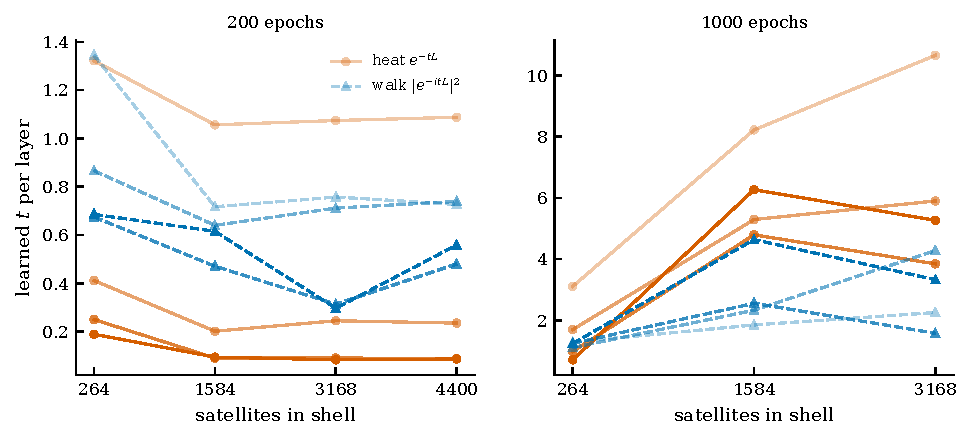
\includegraphics[width=\textwidth]{../figures/out/fig3-t-learned.pdf}
\caption{Learned propagation time per layer (lighter to darker: first to fourth layer) against
shell size, hop field, submitted capacity, softplus arm with $t_{0}=0.5$, mean over valid seeds.
Left: 200 epochs (grid 1). Right: 1000 epochs (grid 2). Note the different vertical scales.}
\label{fig:tlearned}
\end{figure}

\subsection{With enough budget, the heat kernel matches or beats the walk kernel}
\label{sec:budget}

Grid 2 raises the budget to 1000 epochs at the submitted capacity on the three smaller shells.
Every cell now leaves the floor: on the hop field the best operator improves on the constant
predictor by \numGthreeHopsGainMin\% to \numGthreeHopsGainMax\% depending on shell and arm, and on the delay field by \numGthreeDelayGainMin\% to \numGthreeDelayGainMax\%
(Table~\ref{tab:grid3}). The floor of Section~\ref{sec:floor} was a budget floor.

\begin{figure}[t]
\centering
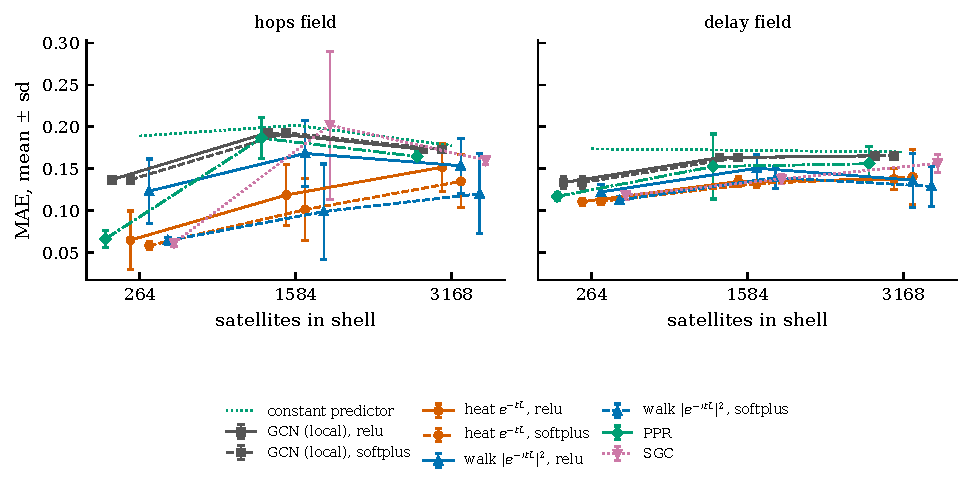
\includegraphics[width=\textwidth]{../figures/out/fig4-scale-1000ep.pdf}
\caption{MAE against shell size at 1000 epochs, submitted capacity, both $t$ arms, both tasks.
Points are means over valid seeds and bars one standard deviation; the dotted line is the
constant predictor. Points are offset horizontally within each shell for legibility.}
\label{fig:scale}
\end{figure}

\begin{table}[t]
\centering
\caption{Grid 2: MAE at 1000 epochs, submitted capacity, mean $\pm$ standard deviation over
valid seeds with the count in parentheses, the number of seeds on which each spectral operator
is lower, and the verdict under rules~3 and~4. ``n$<$7'' marks a cell with too few valid seed
pairs to decide.}
\label{tab:grid3}
% GENERATED by figures/make_figures.py
\begin{tabular}{@{}llrllrl@{}}
\toprule
task & shell & GCN & heat $e^{-tL}$ & walk $|e^{-itL}|^2$ & seeds heat:walk & verdict \\
\midrule
\multicolumn{7}{@{}l}{\emph{hops field, relu, $t_0{=}$0.5}} \\
& 264 & 0.137 & 0.065 $\pm$ 0.035 (9) & 0.123 $\pm$ 0.038 (10) & 8:1 & heat \\
& 1584 & 0.193 & 0.119 $\pm$ 0.037 (6) & 0.168 $\pm$ 0.039 (10) & 4:2 & n$<$7 \\
& 3168 & 0.173 & 0.152 $\pm$ 0.029 (9) & 0.153 $\pm$ 0.033 (9) & 5:3 & tie \\
\multicolumn{7}{@{}l}{\emph{hops field, softplus, $t_0{=}$0.5}} \\
& 264 & 0.137 & 0.058 $\pm$ 0.005 (10) & 0.064 $\pm$ 0.004 (10) & 7:3 & heat \\
& 1584 & 0.193 & 0.101 $\pm$ 0.037 (10) & 0.099 $\pm$ 0.057 (8) & 2:6 & tie \\
& 3168 & 0.173 & 0.135 $\pm$ 0.032 (7) & 0.120 $\pm$ 0.047 (8) & 2:3 & n$<$7 \\
\multicolumn{7}{@{}l}{\emph{delay field, relu, $t_0{=}$0.5}} \\
& 264 & 0.133 & 0.111 $\pm$ 0.004 (10) & 0.122 $\pm$ 0.009 (7) & 7:0 & heat \\
& 1584 & 0.163 & 0.135 $\pm$ 0.006 (10) & 0.151 $\pm$ 0.016 (10) & 8:2 & heat \\
& 3168 & 0.165 & 0.138 $\pm$ 0.012 (10) & 0.136 $\pm$ 0.032 (10) & 6:4 & tie \\
\multicolumn{7}{@{}l}{\emph{delay field, softplus, $t_0{=}$0.5}} \\
& 264 & 0.133 & 0.111 $\pm$ 0.003 (9) & 0.112 $\pm$ 0.004 (10) & 7:2 & heat \\
& 1584 & 0.163 & 0.132 $\pm$ 0.004 (10) & 0.139 $\pm$ 0.013 (10) & 8:2 & heat \\
& 3168 & 0.165 & 0.140 $\pm$ 0.033 (9) & 0.129 $\pm$ 0.024 (7) & 1:5 & n$<$7 \\
\bottomrule
\end{tabular}

\end{table}

Figure~\ref{fig:scale} and Table~\ref{tab:grid3} give the comparison. Under rule~5, the heat
kernel wins robustly at 264 satellites on both tasks and at 1584 satellites on the delay field:
\numGthreeHeatRobust{} of \numGthreeCells{} task-scale cells. The remaining cells are ties or
undecided because pathologies reduced the valid seed count below seven. The walk kernel wins
robustly in \numGthreeWalkRobust{} cells. Where the two are close in mean, they are not close in
variance: on the hop field at 264 satellites in the softplus arm, the heat kernel reaches
\numGthreeHopsSmallHeat{}~$\pm$~\numGthreeHopsSmallHeatSd{} against
\numGthreeHopsSmallWalk{}~$\pm$~\numGthreeHopsSmallWalkSd{} for the walk kernel, with the
constant predictor at \numGthreeHopsSmallConst{}; on the larger shells the walk kernel's
standard deviation across seeds is several times the heat kernel's in most cells. The local
GCN operator is the worst everywhere, as expected for a four-hop model on graphs whose
eccentricity is tens of hops; on the hop field it clears the 5\% floor only on the
264-satellite shell (gain \numGthreeGcnGainSmall\%, against \numGthreeGcnGainShellOne\% at
1584 and \numGthreeGcnGainDouble\% at 3168).

The right panel of Figure~\ref{fig:tlearned} shows what the budget buys. At 1000 epochs the
heat kernel's first-layer $t$ grows with the shell, from \numTlayerOneSmallHeat{} at 264
satellites to \numTlayerOneShellOneHeat{} at 1584 and \numTlayerOneDoubleHeat{} at 3168, while
the walk kernel's stays between \numTlayerOneSmallWalk{} and \numTlayerOneDoubleWalk{}. The
diffusive operator reaches farther on larger graphs by learning to; the walk operator does not
move its time parameter in the same way, and its larger seed variance is consistent with a loss
that is not monotone in $t$.

The preliminary version's finding, a walk-kernel error of \numPrelimWalkMAE{} against
\numPrelimHeatMAE{} at 1584 satellites, is not reproduced. Under the same parameterisation and
capacity, with ten seeds instead of \numPrelimSeeds{}, the two operators tie on the hop field
at that scale and the heat kernel wins on the delay field.

\subsection{Long training collapses a tenth of the runs}
\label{sec:collapse}

Of the \numGridThreeRuns{} runs of grid 2, \numGridThreePathology{}
(\numGridThreePathologyPct\%) were excluded under rule~2. Inspection shows one pattern: the
loss falls, then rises again by up to \numGridThreeRiseMaxPct\% and the run ends on the
constant solution. It affects all three operators and both $t$ arms, and it is the reason
several cells in Table~\ref{tab:grid3} fall below seven valid seed pairs. A fixed learning rate
that is adequate for 200 epochs is not stable for 1000 on these graphs. We report the rate
rather than tune it away, because a reader who runs a longer schedule to escape the floor of
Section~\ref{sec:floor} should expect to meet it.

% =====================================================================
\section{Discussion}
\label{sec:discussion}

\paragraph{Why the probability kernel does not inherit the unitary argument}
The case for walk-based operators in CTQW-GNN~\cite{ctqwgnn} rests on the unitary propagator
acting on feature vectors: it damps no eigencomponent and preserves the Dirichlet energy of the
features across layers. The kernel studied here, and in the preliminary version, is the
transition-probability matrix~\eqref{eq:walk}. It is a real nonnegative row-stochastic matrix,
exactly as the heat kernel is, and applying it to features damps and mixes them in the same way
a diffusion step does. What it inherits from the walk is only the shape of its rows: an
oscillatory profile whose width grows linearly with $t$ rather than as a square root. Once $t$
is a trained parameter, the heat kernel can reach as far by learning a larger $t$, which the
right panel of Figure~\ref{fig:tlearned} shows it does, in the first layer and in proportion to
the shell. The remaining difference is the
profile, and an oscillatory profile makes the loss a non-monotone function of $t$, which is a
plausible source of the larger seed variance the walk kernel shows in Table~\ref{tab:grid3}. A
fair test of the unitary argument on LEO graphs would use the propagator in feature space, as
CTQW-GNN does, and is a different study.

\paragraph{What the floor means for learned propagation on constellations}
A budget that suffices on a 264-satellite shell does not on a 1584-satellite one, and the
failure is silent: the run reports a finite, decreasing loss and an error that looks like a
number. Any comparison of learned propagation across constellation sizes must therefore carry
the constant baseline beside every result and must let the budget grow with the graph, or it
will rank noise. The same holds for comparisons across operator families in which one family
carries a learned reach parameter and the other does not.

\paragraph{What the seed-level bimodality means for reporting}
The split in Figure~\ref{fig:arms} means that a mean over three seeds at this budget is the
mean of a coin flip. The preliminary version's \numPrelimSeeds{}-seed result at 1584 satellites
sits within the range that the bimodality produces, and its direction is the one that
Section~\ref{sec:budget} does not confirm. Ten seeds and a seed-majority rule are the minimum
that made the present cells decidable, and even then the pathology rate of
Section~\ref{sec:collapse} left several undecided.

% =====================================================================
\section{Threats to validity}
\label{sec:threats}

\textbf{The two largest shells are synthetic.} The 3168- and 4400-satellite graphs scale the
Starlink shell-1 geometry and are not deployed constellations. They serve to grow the diameter;
conclusions about them are conclusions about graph size, not about any operator's network.

\textbf{The tasks are node fields, not network functions.} Hop and delay fields isolate
propagation from load, which is what the comparison needs, at the cost of distance from any
routing or traffic-engineering objective. A learned model on a real objective would sit on top
of these operators, and the floor and variance effects would carry over; the ranking might not.

\textbf{One learning rate, one optimiser.} The collapse rate of Section~\ref{sec:collapse} is
specific to Adam at 0.01 for 1000 epochs. A schedule would likely reduce it and might change the
undecided cells. The protocol declares the rate rather than tunes it because tuning per operator
would break parameter matching.

\textbf{The reading rules are choices.} The 5\% floor and the seven-of-ten majority were fixed
before the runs and would give different cell verdicts at other values. Both are reported with
every table so a reader can apply their own.

\textbf{The preliminary artifact does not reproduce its own headline.} The released results of
the preliminary version record \numPrelimParams{} parameters for the 1584-satellite experiment,
which corresponds to the width-32, four-layer network its text describes, while the released
code defaults to width 16 and three layers (\numReleasedParams{} parameters) and contains no
script for that experiment. The preliminary version also ran without the seam cut that its text
states. The present study fixes the seam cut on, runs both capacities, and releases the script
for every number. We state this because the protocol of Section~\ref{sec:protocol} exists to
prevent exactly this class of gap, and it was found by applying the protocol to our own earlier
work.

% =====================================================================
\section{Conclusion}
\label{sec:conclusion}

We asked whether the reported advantage of a quantum-walk probability kernel over the heat
kernel on large LEO inter-satellite-link graphs is a property of the operator. Under a
protocol that matches parameters, shares eigenbases, varies the parameterisation and
initialisation of the learned propagation time, doubles the capacity, raises the budget and
runs ten seeds with declared reading rules, it is not. At the preliminary budget the large
shells are a floor on which no operator learns; at the one shell where learning occurs the
ranking follows the $t$ arm through a seed-level bimodality; and with a budget that clears the
floor, the heat kernel matches or beats the walk kernel wherever the comparison can be decided,
with smaller variance. The practical recommendations are short: carry the constant baseline,
scale the budget with the graph, treat the propagation time as a declared arm, and count
collapsed runs instead of dropping them.

\section*{Data and code availability}
All code, the cached graph instances' construction, every result file of the
\numGridTwelveRuns{} plus \numGridThreeRuns{} runs, the scripts that produce every figure, table
and number in this paper, and the dated protocol declarations are available at
\url{https://github.com/haodpsut/leo-propagation-reach}. The preliminary version and its
released artifact are available at \url{https://github.com/haodpsut/qi-gnn-dynamic-wireless}.

\section*{CRediT authorship contribution statement}
\textbf{Phuc Hao Do:} Conceptualization, Methodology, Software, Investigation, Data curation,
Writing, Visualization.

\section*{Declaration of competing interest}
The author declares no competing interests.

\section*{Declaration of generative AI use}
During the preparation of this work the author used a large language model (Claude, Anthropic)
to assist with code, data analysis scripts and editing of the text. After using this tool, the
author reviewed and edited the content as needed and takes full responsibility for the content
of the publication.

\bibliographystyle{elsarticle-num}
\bibliography{refs}

\end{document}
